\documentclass[a4paper]{scrreprt}
\usepackage[utf8]{inputenc}
\usepackage[ngerman]{babel}
\usepackage[T1]{fontenc}
\usepackage{amssymb}
\usepackage{mathtools}
\usepackage{gensymb}
\usepackage[hyphens]{url}
\usepackage{seqsplit}


\usepackage{graphicx}

\usepackage{geometry}
\geometry{verbose,a4paper,tmargin=25mm,
bmargin=25mm,lmargin=25mm,rmargin=25mm}

\usepackage{float}
\usepackage{enumitem}
\usepackage{hyperref}
\hypersetup{
    colorlinks,
    citecolor=black,
    filecolor=black,
    linkcolor=black,
    urlcolor=black
}


\setlist{nosep} % or \setlist{noitemsep} to leave space around whole list
\setlength\parindent{0pt}


\def\code#1{\texttt{#1}}



\title{Battletanks - Developerhandbuch}
\subtitle{Universität Würzburg Informatik Softwarepraktikum Wintersemester 2016/17}
\author{Armin Bernstetter, Stefan Ernst, Nicolas Fella}

\begin{document}

\maketitle
\tableofcontents
\newpage
\chapter{Pflichtenheft}
\section{Einleitung/Aufgabenstellung}
Mit dem Projekt 'Battletanks' soll ein Desktop-basiertes Multiplayerspiel erstellt werden.
In diesem Spiel können bis zu vier Spieler mit je einer Spielfigur in einem Top Down 2D Spielfeld gegeneinander antreten, indem sie gegnerische Spielfiguren abschießen.
Das Spielfeld kann aus einer externen Datei eingelesen werden.

Das Programm wird für Windows, Linux und Mac OS in Java entwickelt unter Einbezug des Frameworks libGDX und damit auch des Build-Management-Automatisierungs-Tools Gradle.
Die Benutzeroberfläche des Spiels soll hierbei übersichtlich gestaltet werden, 
sodass auch Benutzer ohne jegliches Vorwissen 'Battletanks' spielen können.

\section{Zielbestimmung}
\subsection{Musskriterien}
\subsubsection{Battletanks Game}
\begin{itemize}
\item Lokales Versus-Multiplayer Spiel
\item Bis zu vier Spieler zur selben Zeit
\item Unabhängig von CPU Geschwindigkeit
\item Graphische Benutzeroberfläche
\end{itemize}
\subsubsection{User}
\begin{itemize}
\item Muss ein Spiel starten können
\item Kann Spielfigur im Menü auswählen
\item Hat eine von vier verschiedenen Tastenbelegungen
\item Kann eine Arena laden
\item Kann eine Spieldauer festlegen

\end{itemize}
\subsubsection{GUI}
\subsubsection*{Menü}
\begin{itemize}
\item Per Maus bedienbar
\item Spiel starten
\item Spielfigurauswahl mit Informationen über die Figuren
\item Arena laden 
\item Eingabe der Spieldauer
\end{itemize}

\subsubsection*{Spiel}
\begin{itemize}
\item Enthält Spielfeld und Spielfiguren (Über Tastatur steuerbar)
\item Top-Down 2D Grafik
\item Zeitanzeige
\item Anzeige von Informationen über die Spielfiguren (Leben, Anzahl der Abschüsse)
\end{itemize}


\subsubsection{Spielfigur}
\begin{itemize}
\item Hat eindeutiges Vorne und Hinten
\item Kann sich in 8 Richtungen bewegen ($45\degree$ Drehung möglich)
\item Festgelegte Lebenspunkte
\item Besitzt Waffe (Schussfrequenz, Schaden)
\item Schadensreduzierung
\item Kann Waffe nach vorne abfeuern
\item Bekommt Lebenspunkteabzug falls von gegnerischer Spielfigur getroffen 
\newline Abgezogene Lebenspunkte berechnen sich aus Schaden der gegn. Waffe und der Schadensreduzierung 
\end{itemize}


\subsubsection{Arena/Spielfeldgeometrie}
\begin{itemize}
\item Spielfiguren bewegen sich auf Spielfeld
\item Information über Spielfeld wird aus externer Datei eingelesen
\item Spielfeld enthält Hindernisse
\end{itemize}




\subsection{Abgrenzungskriterien}
\begin{itemize}
\item Keine Netzwerkverbindung benötigt
\item Spiel läuft auf Windows, Linux und Mac OS
\item Keine 3D Grafik
\item Maximal vier Spieler. Einem Spieler ist genau eine Tastenbelegung zugeordnet.

\end{itemize}

\subsection{Kann-Kriterien}
\begin{itemize}
\item Upgrades (Speed-, Damageboost; Streuende Waffen usw)
\end{itemize}

\section{Einsatz}
\subsection{Anwendungsbereiche}
Das Spiel bietet eine Freizeitbeschäftigung, die wenig bis kein Vorwissen und einen benutzerdefinierten Zeitaufwand benötigt. 
\subsection{Zielgruppen}
Personen, die interessiert sind an einem unterhaltsamen und kompetitiven Computerspiel, in dem sie gegen 1-3 Mitspieler antreten können.

\section{Umgebung}
\subsection{Software}
\begin{itemize}
\item Betriebssystem: Windows, Linux oder Mac
\item Java 8
\end{itemize}
\subsection{Hardware}
Beliebiger Computer

\section{Funktionalität}
Typische Anwendung: Das Spiel wird gestartet. Im Menü können die Spieler ihre Spielfiguren auswählen, die Arena aus einer externen Datei einlesen und eine Spieldauer eingeben. Anschließend treten die Spieler gegeneinander an. Die Spieler bewegen ihre Figur mithilfe einer festen Tastenbelegung bestehend aus vier Tasten über ein Spielfeld. Durch Drücken einer zusätzlichen Taste kann die Spielfigur feuern und gegnerische Spielfiguren abschießen, die sich im Schussfeld befinden. Falls die Lebenspunkte einer Spielfigur aufgebraucht sind, wird diese in einer festgelegten/zufälligen (?) Position 'wiederbelebt' und der jeweilige Spieler steigt wieder ins Spiel ein. Der Spieler, der nach Ablauf der Zeit die meisten Abschüsse hat, gewinnt das Spiel.

\section{Benutzeroberfläche}
Benutzeroberfläche bedienbar durch Maus- und Tastatur.
Menü zur Auswahl von Spielfiguren, Spieldauer und Arena. Spielfeld zum Ausführen des Spiels.
\begin{figure}[H]
\textbf{Menu Screen Entwurf:}\par\medskip
\centering
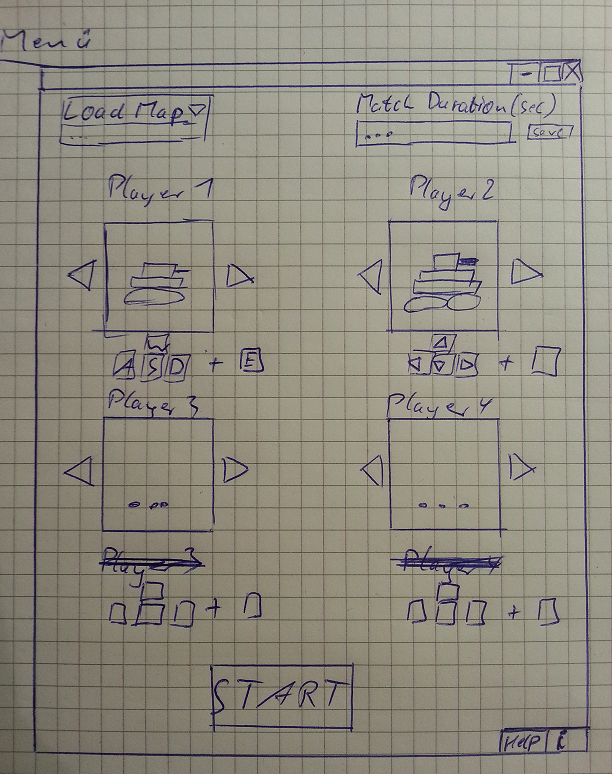
\includegraphics[width=10cm]{menu_entwurf.png}
 \caption{Spielfigur aus Vorschau aller verfügbaren Figuren auswählen. Information über jeweilige Spielfigur verfügbar. Tastenbelegung unter Vorschau angezeigt. Default: Keine Figur ausgewählt, Anzahl Spieler bestimmt durch Anzahl ausgewählter Figuren. Match Duration in Sekunden eingeben}
\end{figure}

\begin{figure}[H]
\textbf{Game Screen Entwurf:}\par\medskip
\centering
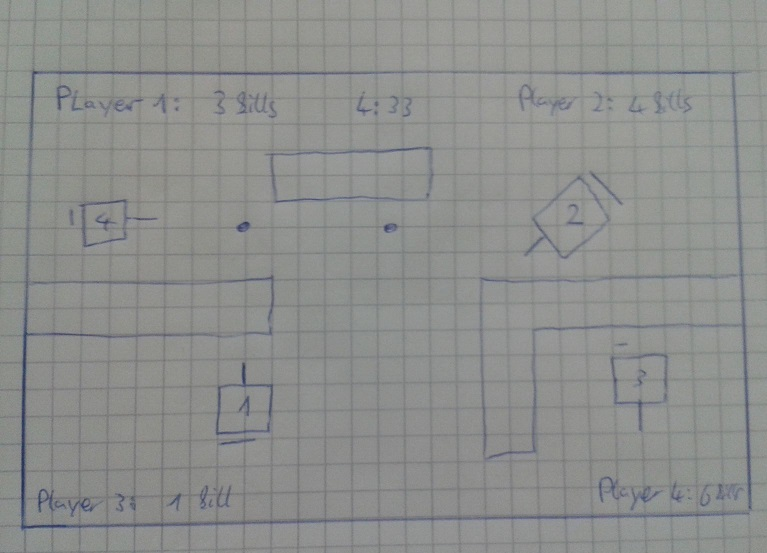
\includegraphics[width=15cm]{game_entwurf.jpg}
\caption{Anzeige der verbleibenden Spielzeit mittig am oberen Spielfeldrand; Anzeige der Abschüsse und Tode der Spieler in den Ecken; Hindernisse, die nicht durchfahren werden können; Spielfiguren feuern Projektile}	
\end{figure}


\section{Qualitätsziele}
\begin{itemize}
\item Spiel läuft flüssig und von der CPU Geschwindigkeit unabhängig
\item Einfache Bedienung durch den Benutzer
\item Figuren leicht steuerbar
\end{itemize}


\chapter{Dokumentation}
\section{Projektaufbau}
\subsection{libGDX}
libGDX (\url{http://libgdx.badlogicgames.com/}) ist ein cross-platform Java-Framework für Spieleentwicklung. Es unterstützt Windows, Linux, Mac OS X, Android, Blackberry, iOS und HTML5.
Es wurde von \href{https://twitter.com/badlogicgames}{\textbf{\textit{Mario Zechner}}} entwickelt und erlaubt dem Programmierer, seinen Code einmal zu schreiben und anschließend auf verschiedenen Plattformen anzuwenden.
LibGDX bietet direkten Zugang zum Dateisystem, zu Eingabe- und Audiogeräten sowie zu OpenGL durch ein kombiniertes OpenGL ES 2.0 und 3.0 interface.
Zusätzlich bietet LibGDX APIs für viele Aufgaben in der Spielentwicklung wie das Rendern von Sprites und Text, UI Erstellung, Soundeffekte und vieles Weiteres.

libGDX benutzt Gradle, ein Build-Management-Automatisierungs-Tool.


\subsection{Einrichten des Projekts}
Um ein libGDX Projekt zu erstellen wird die GDX-Setup App benötigt, die auf der Seite von libGDX zum Download zur Verfügung steht. Anschließend kann man festlegen, für welche Plattformen man entwickeln will und welche Extensions (wie z.B. um Freetype Fonts einlesen/benutzen zu können) man verwenden möchte. Diese können auch nachträglich noch geändert werden durch Änderungen an den build.gradle Dateien. Siehe hierzu die \href{https://github.com/libgdx/libgdx/wiki}{\textbf{\textit{libGDX Wiki}}}.
Im Fall von Battletanks wurde sich auf eine Desktopanwendung beschränkt und die Extensions 'Tools' und 'Freetype' verwendet.

Die Entwicklung geschah größtenteils mit der IDE Eclipse und Java 8, zur Version Control wurde ein Repository auf dem von der Universität Würzburg bereitgestellten Repository Manager \url{https://gitlab2.informatik.uni-wuerzburg.de/} benutzt.



\subsection{Ordnerstruktur}
\subparagraph{Battletanks\_SWP} Dieser Projektordner beinhaltet die von Gradle verwendeted Wrapper- und sonstigen Dateien, einen Ordner 'textures' mit allen verwendeten Grafiken, runnable jar Dateien für das Programm Hiero \url{https://github.com/libgdx/libgdx/wiki/Hiero} zur Umwandlung von TrueTypeFonts in BitMapFonts und einen Texture Packer um die Grafiken in einem 'Texture Atlas' zusammenzufassen.
Zusätzlich befindet sich hier noch ein Ordner mit Benutzer- und Developerhandbuch.

\subparagraph{Battletanks-desktop}
Das  \code{desktop} Projekt beinhaltet nur eine Klasse \code{DesktopLauncher}, die das Spiel als 'Lightweight Java Game Library'-Applikation startet, die eine neue Instanz von \code{BattleTanks} übergeben bekommt.
Damit der \code{DesktopLauncher} auf die richtigen Assets zugreifen kann musste vor der ersten Ausführung das Working Directory in den Run Configurations zum Ordner '\code{Battletanks-core/assets}' geändert werden.

\subparagraph{Battletanks-core}
Dieser Ordner beinhaltet den gesamten Code des Projekts (siehe 2.2 Code), Java Docs sowie alle verwendeten Assets. Darunter befinden sich Soundeffekte, Fonts, die verwendeten TiledMaps, ein UI Skin, Fonts für Menü und Game sowie die Grafiken der Panzer, der Hintergrund und weitere Dateien.



\newpage
\section{Code}
\begin{figure}[H]
  \textbf{Architekturdiagramm:}\par\medskip
  \centering
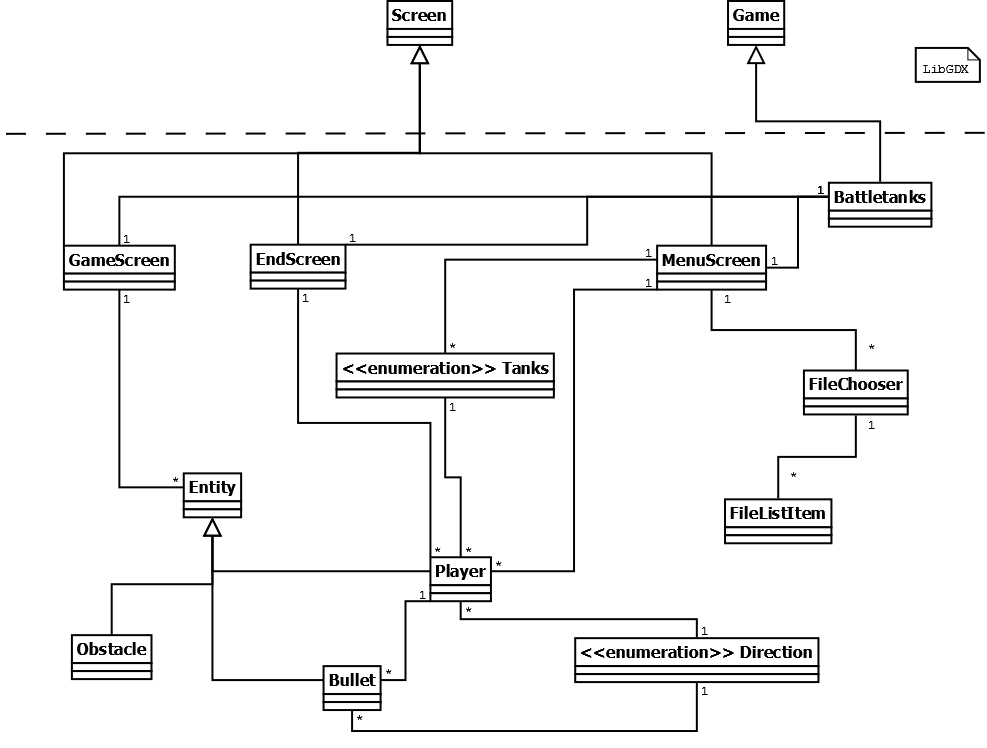
\includegraphics[width=15cm]{architekturdiagramm.png}
\caption{Übersicht über die Klassenstruktur des Projekts}
\end{figure}
\begin{center}\end{center}

\subsection{BattleTanks}
Die Klasse \code{BattleTanks} ist die Hauptklasse. Sie erbt von der LibGDX Klasse \code{Game} und verwaltet die Screens, den TextureAtlas sowie die Preferences/(Vor-)Einstellungen.
Die Methoden \code{showMenu}, \code{showGame} und \code{showEnd} setzen den von der \code{BattleTanks} Instanz angezeigten Screen.

\newpage
\subsection{Package Screens}
Alle Klassen in diesem Package implementieren das LibGDX interface \code{Screen}. Jeder Screen besitzt eine Methode \code{reset}, um z.B. beim mehrmaligen Start neuer Spiele nicht jedes Mal neue Screen Instanzen erstellen zu müssen.
\subsubsection{MenuScreen}
\begin{figure}[H]
  \textbf{Screenshot Menü:}\par\medskip
  \centering
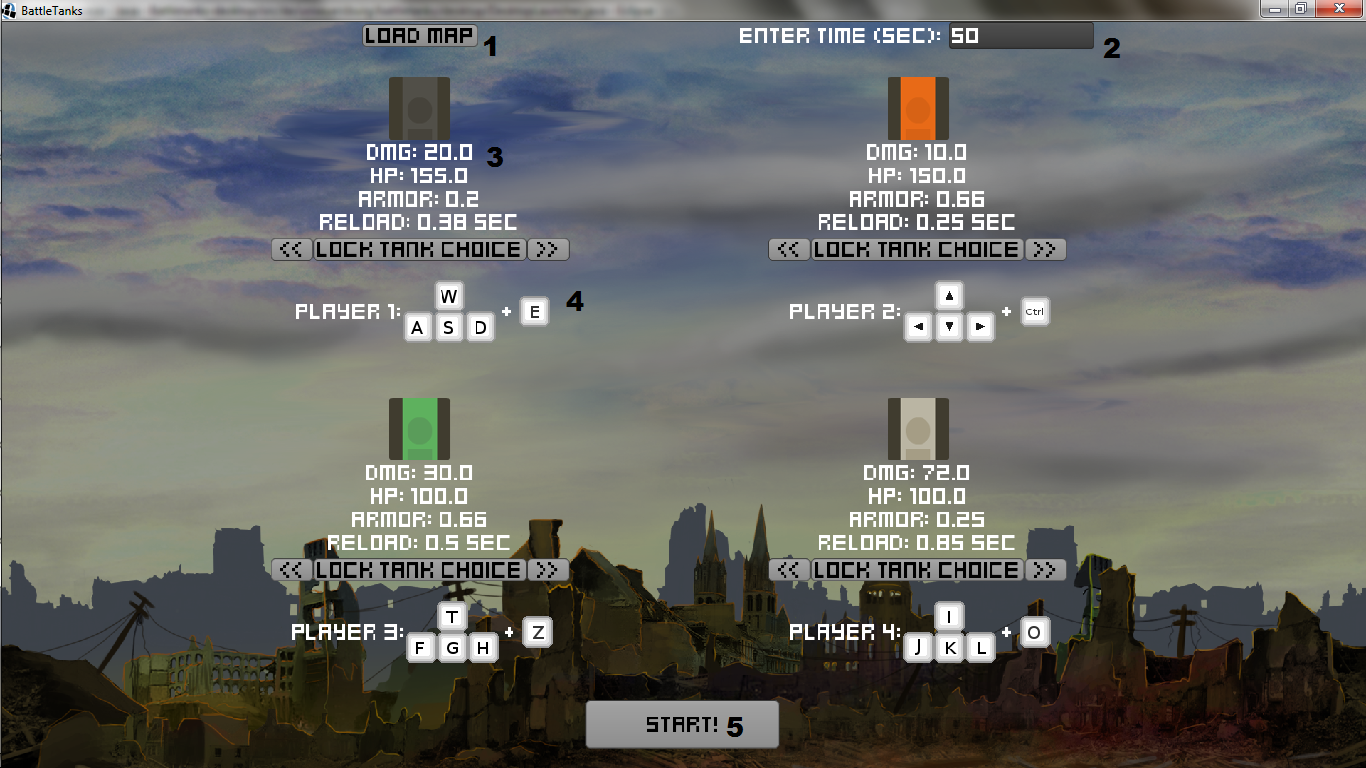
\includegraphics[width=15cm]{screenshot_menu.png}
\caption{1: Map Laden, 2: Zeit Eingeben, 3: Spielfigur auswählen, 4: Tastenbelegung des jew. Spielers,
5: Spiel starten}
\end{figure}


Der \code{MenuScreen} besitzt zwei Stages, auf denen das Menü dargestellt wird. Die Hintergrundstage beinhaltet nur das Hintergrundbild, welches an die Fenstergröße angepasst und bei Bedarf gestreckt/gestaucht wird.
Das gesamte Menü wird durch die zweite Stage dargestellt, die eine Table \code{mainTable} beinhaltet, auf der sich alle UI Elemente befinden. Diese werden jeweils von Methoden erstellt, die nach dem Schema '\code{createUIElement()}' benannt sind und werden anschließend von der Methode '\code{create()}' auf der mainTable angeordnet.


Zur Darstellung aller UI Elemente wird der im Ordner \code{assets/data} befindliche Skin \code{uiskin.json} verwendet. (Siehe 2.3.3 Skin/Fonts)

Wurden alle notwendigen Informationen vom Benutzer eingegeben, wird durch Aufruf der \code{showGame()} Methode der Klasse \code{BattleTanks} das Spiel gestartet indem zu einem \code{GameScreen} gewechselt wird.


\newpage
\subsubsection{GameScreen}
\begin{figure}[H]
  \textbf{Screenshot Game:}\par\medskip
  \centering
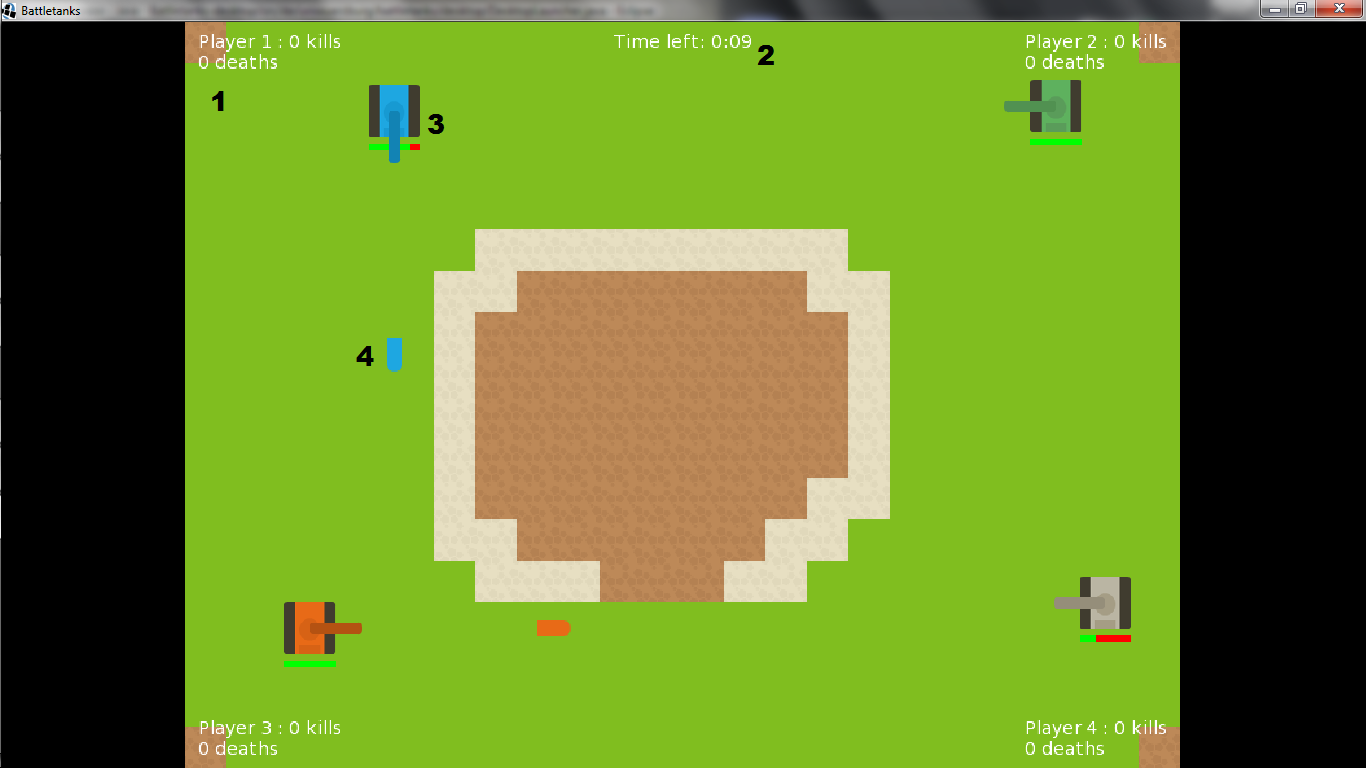
\includegraphics[width=15cm]{screenshot_game.png}    \caption{1: Anzeige von Abschüssen und Toden, 2: Verbleibende Spielzeit, 3: Panzer mit Kanone nach unten ausgerichtet, 4: Projektil des blauen Panzers}
\end{figure}
Im \code{GameScreen} befindet sich die gesamte Spiellogik. Der Konstruktor bekommt eine Liste von Spielern, die Spieldauer und den Dateipfad der ausgewählten Map übergeben.
Letzterer wird in der Methode \code{loadMap} verwendet, um die Map aus der .tmx Datei einzulesen (Siehe 2.3.1 Die Maps).
Die Methode \code{render} wird in jedem Frame aufgerufen und aktualisiert das gesamte Spiel, also alle Entities, die sich auf dem Spielfeld befinden, alle Textanzeigen und die Map.

\subparagraph{Kollisionserkennung} Grundsätzlich können sich die Player jeden Frame beliebig bewegen. Bevor die neuen Positionen allerdings gezeichnet werden, findet die Kollisionserkennung und -auflösung statt. Zur Erkennung besitzt jede Entity ein Kollisionsrechteck, welches verwendet wird, um zu überprüfen, ob sich zwei Entities überschneiden. Falls dies der Fall ist, wird die Überlappung in x- und y-Richtung berechnet. Je nachdem, welcher Wert kleiner ist, wird die Kollision in der entsprechenden Richtung wieder aufgelöst.

Hierbei dient die Geschwindigkeit der beiden Entities dazu, den Typ der Kollision festzustellen. Falls eine der beiden Entities steht (Beispiel: Player-Obstacle-Kollisionen), wird die sich bewegende Entity ausgebremst und an den Rand der anderen zurückgesetzt. 

Ein weiterer Kollisionstyp findet statt, falls beide Entities aufeinander zufahren. Dies wird aufgelöst, indem die Entities jeweils zur Hälfte der Überlappung zurückgesetzt werden. Zuletzt könnte es noch sein, dass die eine Entity langsamer war als die andere, sodass letztere der anderen hinten auffährt. In diesem Fall wird die schnellere ausgebremst und an den Rand der anderen zurückgesetzt. Zusätzlich wird die Geschwindigkeit der versetzten Entities in der entsprechenden Richtung auf 0 gesetzt, sodass sie bei einer weiteren Kollision nicht als Kollisionsverursacher wieder entlang dieser Richtung verschoben werden können.


Damit die Player zuerst von den Wänden weggeschoben werden, findet als Erstes die Kollisionserkennung zwischen Playern und Obstacles und anschließend die zwischen Playern und Playern statt. Die Kollisionen zwischen Bullets und Entities werden zuletzt überprüft und löschen die Bullets (mit Schaden bei Playern).
\newpage
\subsubsection{EndScreen}
\begin{figure}[H]
  \textbf{Screenshot Scoreboard:}\par\medskip
  \centering
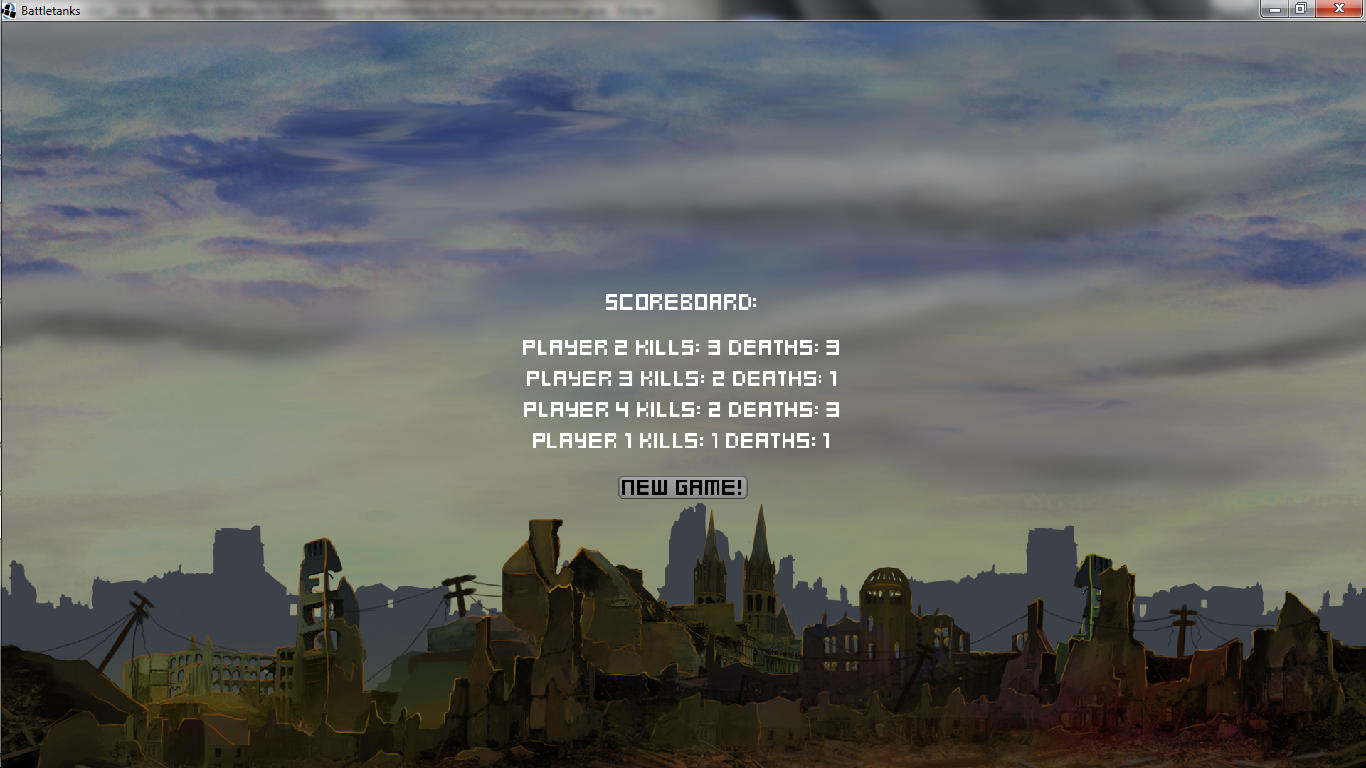
\includegraphics[width=15cm]{screenshot_endscreen.png}    
\caption{Spielende und Starten eines neuen Spiels}
\end{figure}
Der \code{EndScreen} erscheint sobald die eingegebene Zeit abgelaufen ist. Er ist ähnlich aufgebaut wie der \code{MenuScreen} mit einer Main Stage und Background Stage und bekommt eine Liste an Playern übergeben. Diese werden mithilfe des internen \code{PlayerComparator} zuerst absteigend nach Kills, aufsteigend nach Deaths und danach aufsteigend nach \code{PlayerNumber} sortiert und in Form eines Scoreboards dargestellt. Zudem besitzt \code{EndScreen} einen Button, mit dem ein neues Spiel gestartet werden kann.


\subsubsection*{ErrorScreen}
Der \code{ErrorScreen} erscheint zum aktuellen Stand des Programmes nur, wenn eine Map geladen wurde, auf der die Spielfiguren unmittelbar auf Hindernissen spawnen.
Er ist an das Design des \code{EndScreen} angelehnt und zeigt nur eine Fehlermeldung, die beim Aufruf des Konstruktors übergeben werden kann sowie einen 'New Game' Button.

\newpage
\subsection{Package Entity}
\subparagraph{Entity}
Die Klasse \code{Entity} implementiert das libGDX Interface \code{Disposable}. Dies bedeutet, dass Instanzen dieser Klasse am Ende ihrer Lebenszeit manuell 'disposed' werden müssen, da es sonst zu Memory Leaks kommen kann. 
Jede Instanz einer Entity besitzt eine Position im Koordinatensystem, eine Höhe und Breite sowie eine 2D Sprite, die aus dem \code{TextureAtlas} ausgelesen wird.
Zusätzlich hat jede Instanz ein '\code{collisionRectangle}' und eine Koordinate, die zur Kollisionsberechnung verwendet werden.


\subparagraph{Player}
Die Klasse \code{Player} erbt von \code{Entity}. Sie stellt eine Spielfigur mit einem \code{Tank} (siehe Enum Tanks), einer Tastenbelegung, einer Spielernummer, einer Bewegungsgeschwindigkeit und einer 2D Sprite 'Gun' dar. Die Player eines Spiels werden bereits im MenuScreen erstellt wenn der 'Lock Tank Choice'-Button gedrückt wird und werden dann an den GameScreen übergeben.

Die Methode \code{update()} verarbeitet u.a. mit Aufruf mehrerer Untermethoden die Benutzereingaben und bewegt die Spielfigur bzw erzeugt ein neues Projektil. Zudem kümmert sich diese Methode um den Respawn des Spielers.
\subparagraph{Bullet}
Die Klasse \code{Bullet} erbt von Entity. Bullets gehören zu einer Player Instanz. Dies wird benötigt um zu berechnen, welcher Player einen anderen abgeschossen hat.
\subparagraph{Obstacle}
Die Klasse \code{Obstacle} erbt ebenfalls von Entity. Sie stellt ein Hindernis auf der Map dar.
\subparagraph{Enum Direction}
\code{Direction} ist ein Enum, das die 8 möglichen Richtungen darstellt, in die sich eine Spielfigur bewegen kann.

\subparagraph{Enum Tanks}
Das Enum \code{Tanks} erstellt die fünf Spielfiguren. Jede davon besitzt einen Damage- Armor- und HealthPoints-Wert sowie eine ReloadTime/Schussfrequenz. 

\newpage
\subsection{Package Utility}
\subparagraph{FileChooser}
\begin{figure}[H]
  \textbf{Screenshot FileChooser:}\par\medskip
  \centering
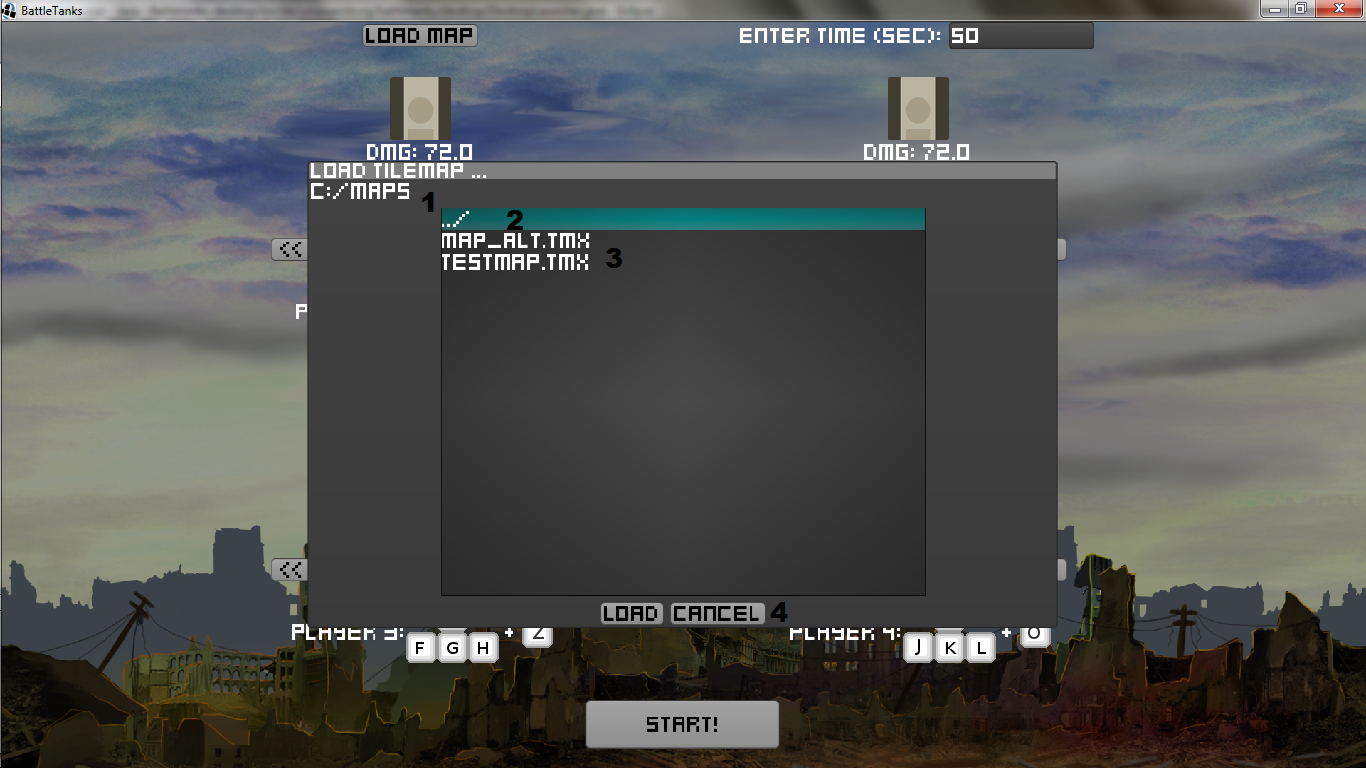
\includegraphics[width=15cm]{screenshot_filechooser.png}  
\caption{1: Anzeige des aktuellen Ordnerpfades, 2: Wechseln in den vorherigen Ordner, 3: Die zur Auswahl stehenden Maps, 4: Ausgewählte Map laden oder Abbrechen}
\end{figure}

Der \code{FileChooser} wurde benötigt, da LibGDX kein Fenster zur Auswahl einer Datei enthält und basiert grundlegend diesem Entwurf (\url{http://www.java-gaming.org/index.php?topic=35471.0}).
Er erbt von der Klasse \code{Dialog}, welche bereits Methoden zum Hinzufügen von Buttons, Ausgeben eines Resultats und Anzeigen eines Dialogfensters bietet. Der \code{FileChooser} enthält Buttons zum Laden und zum Abbrechen der Mapauswahl. Des Weiteren wird dem Dialogfenster eine \code{ScrollPane} hinzugefügt, die wiederum aus einer Liste von \code{FileListItems} besteht. Die Elemente der Liste entsprechen den Ordnern und Dateien wobei letztere nach Dateiendung .tmx gefiltert werden und Ordner vor Dateien angezeigt werden. Beim Klick auf eines der Elemente wird entweder der Ordner gewechselt und dessen Inhalt angezeigt oder die Datei ausgewählt. Zum Erstellen eines \code{FileChoosers} wird eine statische Methode verwendet, in der die \code{result} Methode so überschrieben wird, dass das Ergebnis der \code{result} Methode eines selbst definierten \code{ResultListeners}, dessen Interface im \code{FileChooser} enthalten ist, übergeben wird. Dieser \code{ResultListener} kann außerdem mit einer weiteren Methode gesetzt werden um festzulegen, was beim Schließen des Fensters passieren soll. Die ausgewählte Datei kann zum Schluss mit einer weiteren Methode abgefragt werden.

\subparagraph{FileListItem}
Diese Klasse wird benötigt um die Liste von Ordnern und Dateien im \code{FileChooser} zu realisieren. Ein \code{FileListItem} entspricht grundsätzlich einem Ordner bzw. einer Datei, enthält jedoch zusätzlich noch einen Namen, dem bei Ordnern noch ein '/' zur Unterscheidung angehängt wird. Die \code{toString} Methode wird außerdem so überschrieben, dass hierbei der Name zurückgegeben wird.

\newpage
\section{Dateien/Assets}
\subsection{Die Maps}
Zum Einlesen von Maps wird eine Datei im TMX Format (\url{http://doc.mapeditor.org/reference/tmx-map-format/}) benötigt. Diese enthält die erstellte Map mit Verweis auf Grafiken in Form eines Tilesets und kann aus mehreren Layers bestehen. Die Größe der Map ist egal, da das Spiel entsprechend skaliert wird. Zu beachten ist jedoch, dass die Tanks standardmäßig eine Größe von 40x40 Pixel haben und in den Ecken spawnen müssen. Der Rest der Map kann beliebig gestaltet werden. Damit die Obstacles jedoch eingelesen werden können, muss eine Objektebene namens 'objects' existieren, die alle Hindernisse als rechteckige Objekte enthält. Diese werden dann intern in Obstacles übersetzt, während die restlichen Layers nur als Hintergrund dienen.
Es bietet sich außerdem an, die Tilemap mithilfe eines Editors, wie zum Beispiel dem Tiled Map Editor (\url{http://www.mapeditor.org/}) zu erstellen.


\subsection{Textures/Grafiken}
Der Großteil der verwendeten Grafiken wurde auf \url{http://opengameart.org/} gefunden.
Das Hintergrundbild stammt von 
\url{https://mobilegamegraphics.com/product/airplane-dogfight-assets-free-assets/} und sämtliche im Game verwendeten Textures wurden erstellt von \url{http://kenney.nl/assets/topdown-tanks}. Dies beinhaltet die Textures aus denen die Default-Map besteht, die Bullets sowie Panzer.

\subsection{Skin/Fonts}
Der verwendete \code{Skin} in Form einer .json Datei sowie alle zugehörigen Dateien befinden sich im Ordner \code{assets/data} im \code{core} Projekt. Ausgenommen des im Menü und EndScreen verwendeten Fonts \code{pixel.fnt} stammen die verwendeten Dateien aus dem libGDX Tests Repository \url{https://github.com/libgdx/libgdx/tree/master/tests/gdx-tests-android/assets/data} und werden in der libGDX Dokumentation als default Dateien zur Verwendung empfohlen. Zur näheren Information über die Funktionsweise von Skins siehe \url{https://github.com/libgdx/libgdx/wiki/Skin}

Der Font \code{pixel.fnt} stammt ebenfalls von \url{http://kenney.nl/assets/kenney-fonts} und wurde mithilfe des Programms Hiero von einem TrueTypeFont in einen BitMapFont umgewandelt.

\subsection{Sounds}
Sowohl der Schuss-Soundeffekt als auch die standardmäßig auskommentierte Hintergrundmusik wurden auf \url{http://www.freesound.org/} gefunden.

Soundeffekt: \url{http://www.freesound.org/people/ShawnyBoy/sounds/166191/}

Musik: \url{http://www.freesound.org/people/Airwolf89/sounds/346455/}

\newpage
\section{Tests}
\subsection{JUnit Tests}
Das Package  \code{de.uniwuerzburg.battletanks.test} enthält Unit-Tests für die Klassen aus dem Package \code{Entity} (Siehe 2.2.3). Hierfür wird JUnit4 eingesetzt. Um die Unit-Tests zu ermöglichen werden einzelne Funktionen von libGDX von den Klassen in \seqsplit{\code{de.uniwuerzburg.battletanks.test.mock}} imitiert. Hierfür ist es wichtig, dass zu Beginn der Test eine Instanz von \code{MockBattleTanks} erstellt wird. Dies wird beim ausführen der Test-Suite \code{AllTests} getan. Beim Ausführen einzelner Tests muss dies manuell geschehen. Die anderen Komponenten von Battletanks lassen sich aufgrund der komplexen Zusammenhänge von graphischer Oberfläche, OpenGL, Spielmechanik, libGDX und Benutzereingaben nicht mit Unit-Tests testen. Hierfür existiert ein Test-Protokoll. 

\subsection{Testprotokoll}
Da die JUnit Tests viele Bereiche der GUI nicht abdecken können, soll das folgende Protokoll die restlichen Tests enthalten. In diesem Testprotokoll werden verschiedene mögliche Fehlerquellen angegeben und deren Überprüfung beschrieben.

\subsubsection*{MenuScreen}
\subparagraph*{Fehlerquelle:}
Bei der Eingabe einer Spielzeit könnten Probleme entstehen, wenn der Nutzer zum Beispiel negative Zahlen oder Buchstaben eingibt.
\subparagraph*{Test:}
Im Test wurde die Zeit auf 'ABC' gesetzt, Spieler ausgewählt und das Spiel gestartet. Daraufhin öffnete sich ein Fenster mit dem Hinweis 'NO VALID TIME ENTERED!'. Mit dem Zeitwert '-60' startete das Spiel jedoch und der Betrag der Zahl wurde als Spielzeit gewählt.
		
\subparagraph*{Fehlerquelle:}
Beim Einlesen von Maps könnte häufiges Wechseln der Map die alte Map nicht überschreiben oder falsche Namen anzeigen. 
\subparagraph*{Test:}
Im Test wurde eine Map geladen, deren Name anschließend neben dem 'LOAD MAP' Button erschien. Als erneut eine Map ausgewählt wurde, änderte sich auch der Schriftzug und beim Spielstart wurde letztere auch richtig geladen. 

\subparagraph*{Fehlerquelle:}
Eine fehlerhafte Map könnte das Spiel zum Absturz bringen.
\subparagraph*{Test:} 
Im Test wurde deshalb eine leere Datei 'map.tmx' erstellt und anschließend geladen. Nach Auswahl der Spieler und Starten des Spiels traten keinerlei Fehler auf und die Standard-Map wurde geladen.
		
\subparagraph*{Fehlerquelle:}
Bei der Auswahl der Tanks könnten die Buttons falsch zugewiesen worden sein oder Spielern nicht alle Tanks zur Verfügung stehen.
\subparagraph*{Test:}
Aus diesem Grund wurden im Test bei jedem Spieler alle Tanks rückwärts und vorwärts durchgeschaltet. Dies funktionierte ohne Probleme und bei jedem Spieler waren alle Tanks verfügbar. 

\subparagraph*{Fehlerquelle:}
Ein weiteres Problem könnte das Tankwechseln nach dem betätigen des Lock-Buttons sein. 
\subparagraph*{Test:}
Hierbei wurde für jeden Spieler ein Tank 'gelockt' und dann versucht, den Tank in beide Richtungen zu ändern. Das Ergebnis zeigte, dass die Lock-Buttons richtig implementiert wurden.

\subparagraph*{Fehlerquelle:}
Außerdem könnte es beim Spielstart passieren, dass ein Spieler den falschen Tank erhält. 
\subparagraph*{Test:}
Dies wurde getestet indem jeder Spieler einen anderen Tank erhielt und alle gelockt wurden. Beim Spielstart zeigte sich, dass jeder Spieler auch den richtigen Tank steuerte.
		
\subparagraph*{Fehlerquelle:}
Des Weiteren musste getestet werden, was bei einem Spielstart mit zu wenig oder fehlerhaften Einstellungen passiert. 
\subparagraph*{Test:}
Hierzu wurde versucht das Spiel ohne gelockten Tank zu starten. Das Ergebnis war ein Fenster mit dem Hinweis 'NO TANK CHOSEN!'. Versuchte man das Spiel z.B. mit '1F?' als Zeit zu starten, erschien hingegen der Hinweis 'NO VALID TIME ENTERED!'. 

\subsubsection*{FileChooser}
\subparagraph*{Fehlerquelle:}
Bei der Verwendung des FileChoosers könnte es passieren, dass der Nutzer beliebige Dateien einliest. Auch die Navigation durch Verzeichnisse könnte nicht ordentlich funktionieren. 
\subparagraph*{Test:}
Bei dem Versuch, eine falsche Datei einzulesen zeigte sich, dass dies nicht möglich ist, da die Dateien von vornherein nach Dateiendung '.tmx' gefiltert wurden. Um die Ordnernavigation zu testen wurde hierbei versucht in diverse Verzeichnisse zu wechseln und diese auch wieder zu verlassen. Dies funktionierte ohne Probleme, da immer der richtige Ordner geöffnet wurde. Anschließend wurde das Auswählen und Bestätigen einer Datei getestet. Hierbei wurde auf den Desktop navigiert und anschließend eine Datei 'map.tmx' durch einen Klick ausgewählt. Beim Bestätigen mit dem 'LOAD' Button wurde der richtige Dateiname an das Menü übergeben und beim Spielstart auch geladen. Nun wurde noch die Funktion des 'CANCEL' Buttons getestet. Es wurde zunächst eine Map eingelesen und dann ein weiteres Mal der FileChooser geöffnet. Die Verzeichnisse wurden gewechselt und zum Schluss eine andere Map ausgewählt, jedoch dann auf 'CANCEL' gedrückt. Im Menü stand anschließend immer noch der alte Mapname und beim Spielstart wurde diese auch korrekt geladen.
		
\subsubsection*{GameScreen}
\subparagraph*{Fehlerquelle:}
Im GameScreen musste sicher gestellt werden, dass die Tasten zur Steuerung der Tanks auch immer die richtige Spielfigur steuern und alle funktionierten. 
\subparagraph*{Test:}
Im Test wurde hierzu ein Spiel mit vier Spielern erstellt und jeder Tank in alle Richtungen bewegt und geschossen. Es traten keinerlei Probleme auf und jeder Tank hatte die gleichen Funktionalitäten. In einem weiteren Test wurde überprüft, ob die Kugeln beim Schießen in eine beliebige Richtung immer am Ende des Panzerrohrs spawnen. Auch hierbei traten keine Fehler auf. Des Weiteren wurde getestet, ob sich sowohl Panzer als auch Kugeln mit konstanter Geschwindigkeit bewegen. Dieser Test erfolgte mit Augenmaß und durch den Vergleich paralleler Kugeln und Panzern.
		
\subparagraph*{Fehlerquelle:}
Auch die Kollisionen von Kugeln mit anderen Objekten könnten nicht immer das erwünschte Ergebnis geben. 
\subparagraph*{Test:}
Im Test wurden hierzu einige Kugeln aus unterschiedlichsten Richtungen auf ein Hindernis geschossen. Alle Kugeln wurden unverzüglich nach dem Aufprall gelöscht. Bei Kollisionen mit anderen Spielern musste zusätzlich überprüft werden, ob diese auch entsprechenden Schaden nehmen. Dabei wurden von jedem Tank Kugeln auf andere Tanks abgefeuert. Der Schaden wurde immer korrekt vom Leben abgezogen und beim Sinken der Lebensanzeige auf 0, wurden zusätzlich die Kill- und Death-Counter korrekt erhöht.
		
\subparagraph*{Fehlerquelle:}
Sehr wichtig sind auch die Kollisionen der Tanks mit anderen Objekten und dass diese auch realistisch sowie fehlerfrei aufgelöst werden. 
\subparagraph*{Test:}
Beim ersten Test wurde versucht mit den Tanks das Spielfeld zu verlassen. Die Ränder verhielten sich hierbei wie Wände, durch die der Tank nicht fahrn konnte. In einem weiteren Test erfolgten dann Kollisionen mit Hindernissen, indem von allen Richtungen auf diese zugefahren wurde. Diese Kollisionen verliefen größtenteils sehr gut, sodass die Tanks nie die Hindernisse durchdringen konnten. Lediglich in wenigen Fällen, in denen der Tank diagonal die Ecken von Hindernissen streifte, verlief die Kollision etwas unnatürlich. In einem letzten Test wurden die komplexeren Kollisionen zwischen zwei sich bewegenden Tanks getestet. Dies geschah indem alle vier Spieler auf engem Raum aufeinander zufuhren. Auch hierbei kam es zu fast keinen Problemen. Nur in seltenen Fällen verursachten die vielen Kollisionen kleine, unnatürliche Sprünge der Tanks.
		
\subparagraph*{Fehlerquelle:}
Inkorrekter Ablauf der Spielzeit.
\subparagraph*{Test:}
Dies wurde getestet, indem die Spieldauer mit der aus dem Menü verglichen wurde und geprüft wurde ob sie sich im Sekundentakt verringert. Dies funktionierte ohne Probleme und nach Ablauf der Zeit wechselte das Spiel automatisch zum EndScreen.
		
\subsubsection*{EndScreen}
\subparagraph*{Fehlerquelle:}
Im EndScreen könnten falsche oder unbeteiligte Spieler gezeigt werden oder die Sortierung nicht der Platzierung der Spieler entsprechen. 
\subparagraph*{Test:}
Deswegen wurden mehrmals die Ergebnisse und Spieler eines Spiels notiert und mit den Werten im EndScreen verglichen. Auch die Sortierung nach der Anzahl an Kills wurde überprüft. Hierbei zeigten sich keinerlei Fehler. Zuletzt wurde die Funktionalität des 'NEW GAME' Buttons überprüft. Beim Betätigen wechselte das Spiel erfolgreich in den MenuScreen, in dem die Einstellungen für ein weiteres Spiel gemacht werden konnten.



\end{document}